\documentclass[tikz,border=12pt]{standalone}
\usepackage[T1]{fontenc}
\usepackage{lmodern,amsmath,amssymb}
\usetikzlibrary{arrows.meta,positioning}
\definecolor{ink}{HTML}{183444}
\definecolor{blue}{HTML}{1B6780}
\definecolor{amber}{HTML}{AD601A}
\begin{document}
\hyphenpenalty=10000\exhyphenpenalty=10000
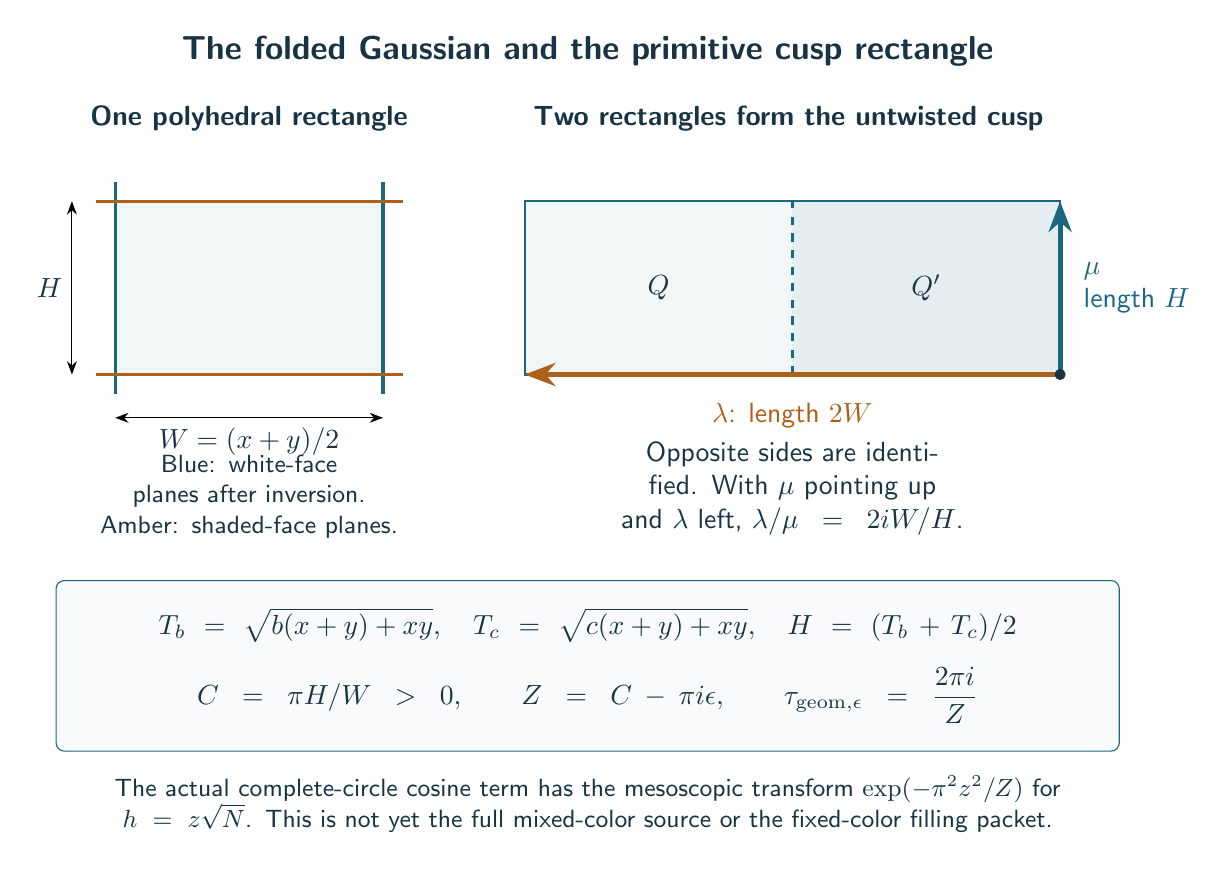
\begin{tikzpicture}[font=\sffamily,text=ink,>=Stealth]
 \node[font=\sffamily\large\bfseries] at (6,4.1)
 {The folded Gaussian and the primitive cusp rectangle};
 \node[font=\sffamily\bfseries] at (1.7,3.25)
 {One polyhedral rectangle};
 \fill[blue!6] (0,0) rectangle (3.4,2.2);
 \draw[blue,very thick] (0,-.25)--(0,2.45) (3.4,-.25)--(3.4,2.45);
 \draw[amber,very thick] (-.25,0)--(3.65,0) (-.25,2.2)--(3.65,2.2);
 \draw[<->] (0,-.55)--node[below] {$W=(x+y)/2$} (3.4,-.55);
 \draw[<->] (-.55,0)--node[left] {$H$} (-.55,2.2);
 \node[align=center,font=\sffamily\small,text width=4.1cm] at (1.7,-1.55)
 {Blue: white-face planes after inversion.\\
 Amber: shaded-face planes.};

 \node[font=\sffamily\bfseries] at (8.55,3.25)
 {Two rectangles form the untwisted cusp};
 \fill[blue!6] (5.2,0) rectangle (8.6,2.2);
 \fill[blue!12] (8.6,0) rectangle (12,2.2);
 \draw[blue,thick] (5.2,0) rectangle (12,2.2);
 \draw[blue,dashed,thick] (8.6,0)--(8.6,2.2);
 \node at (6.9,1.1) {$Q$};
 \node at (10.3,1.1) {$Q'$};
 \draw[->,amber,line width=1.8pt] (12,0)--(5.2,0);
 \draw[->,blue,line width=1.8pt] (12,0)--(12,2.2);
 \fill[ink] (12,0) circle (2pt);
 \node[amber,below=7pt] at (8.6,0) {$\lambda$: length $2W$};
 \node[blue,right=5pt,align=left] at (12,1.1) {$\mu$\\length $H$};
 \node[align=center,text width=7.2cm] at (8.6,-1.45)
 {Opposite sides are identified. With $\mu$ pointing up\\
 and $\lambda$ left, $\lambda/\mu=2iW/H$.};

 \node[draw=blue,rounded corners=3pt,fill=blue!3,
       align=center,text width=12.8cm,inner sep=10pt] at (6,-3.7)
 {$T_b=\sqrt{b(x+y)+xy},\quad T_c=\sqrt{c(x+y)+xy},\quad
 H=(T_b+T_c)/2$\\[8pt]
 $C=\pi H/W>0,\qquad
 Z=C-\pi i\epsilon,\qquad
 \tau_{\mathrm{geom},\epsilon}=\dfrac{2\pi i}{Z}$};
 \node[align=center,text width=13.3cm,font=\sffamily\small] at (6,-5.45)
 {The actual complete-circle cosine term has the mesoscopic transform
 $\exp(-\pi^2 z^2/Z)$ for $h=z\sqrt N$.
 This is not yet the full mixed-color source or the fixed-color filling packet.};
\end{tikzpicture}
\end{document}
